%% Template for Stata-Journal Quarto manuscript

%% Main

% main.tex - a driver for your Stata Journal insert
% This file should only be changed according to the AUTHOR notes below.
% The Stata Press document class

\documentclass[bib]{statapress}

% Page dimensions
\usepackage[crop,newcenter,frame]{pagedims}
% The Stata Journal styles
\usepackage{sj}
% Stata Log listings and useful macros
\usepackage{stata}
% Encapsulated PostScript figures
\usepackage{epsfig}
% Shadow package to render technical note figure
\usepackage{shadow}
\usepackage{amsmath,amssymb} 
% EDITORS: volume number, issue number, month, and year
\usepackage{setspace}
%% Hide Links
%CodeThis is for Executed code. But may not be necessary
\usepackage{color}
\usepackage{fancyvrb}
\newcommand{\VerbBar}{|}
\newcommand{\VERB}{\Verb[commandchars=\\\{\}]}
\DefineVerbatimEnvironment{Highlighting}{Verbatim}{commandchars=\\\{\}}
% Add ',fontsize=\small' for more characters per line
\usepackage{framed}
\definecolor{shadecolor}{RGB}{255,255,255}
\newenvironment{Shaded}{\begin{snugshade}}{\end{snugshade}}
\newcommand{\KeywordTok}[1]{\textcolor[rgb]{0.00,0.0,0.0}{#1}}
\newcommand{\NormalTok}[1]{\textcolor[rgb]{0.00,0.0,0.0}{#1}}




%% Ref

 

\sjsetissue{vv}{ii}{mm}{yyyy}

%%%%%%%%%%%%%%%%%%%%%%%%%%%%%%%%%%%%%%%%%%%%%%%%%%%%%%%%%%%%%%%%%%%%%%%%%%%%%%%


\providecommand{\tightlist}{%
  \setlength{\itemsep}{0pt}\setlength{\parskip}{0pt}}\usepackage{longtable,booktabs,array}
\usepackage{calc} % for calculating minipage widths
% Correct order of tables after \paragraph or \subparagraph
\usepackage{etoolbox}
\makeatletter
\patchcmd\longtable{\par}{\if@noskipsec\mbox{}\fi\par}{}{}
\makeatother
% Allow footnotes in longtable head/foot
\IfFileExists{footnotehyper.sty}{\usepackage{footnotehyper}}{\usepackage{footnote}}
\makesavenoteenv{longtable}
\usepackage{graphicx}
\makeatletter
\newsavebox\pandoc@box
\newcommand*\pandocbounded[1]{% scales image to fit in text height/width
  \sbox\pandoc@box{#1}%
  \Gscale@div\@tempa{\textheight}{\dimexpr\ht\pandoc@box+\dp\pandoc@box\relax}%
  \Gscale@div\@tempb{\linewidth}{\wd\pandoc@box}%
  \ifdim\@tempb\p@<\@tempa\p@\let\@tempa\@tempb\fi% select the smaller of both
  \ifdim\@tempa\p@<\p@\scalebox{\@tempa}{\usebox\pandoc@box}%
  \else\usebox{\pandoc@box}%
  \fi%
}
% Set default figure placement to htbp
\def\fps@figure{htbp}
\makeatother

\makeatletter
\@ifpackageloaded{caption}{}{\usepackage{caption}}
\AtBeginDocument{%
\ifdefined\contentsname
  \renewcommand*\contentsname{Table of contents}
\else
  \newcommand\contentsname{Table of contents}
\fi
\ifdefined\listfigurename
  \renewcommand*\listfigurename{List of Figures}
\else
  \newcommand\listfigurename{List of Figures}
\fi
\ifdefined\listtablename
  \renewcommand*\listtablename{List of Tables}
\else
  \newcommand\listtablename{List of Tables}
\fi
\ifdefined\figurename
  \renewcommand*\figurename{Figure}
\else
  \newcommand\figurename{Figure}
\fi
\ifdefined\tablename
  \renewcommand*\tablename{Table}
\else
  \newcommand\tablename{Table}
\fi
}
\@ifpackageloaded{float}{}{\usepackage{float}}
\floatstyle{ruled}
\@ifundefined{c@chapter}{\newfloat{codelisting}{h}{lop}}{\newfloat{codelisting}{h}{lop}[chapter]}
\floatname{codelisting}{Listing}
\newcommand*\listoflistings{\listof{codelisting}{List of Listings}}
\makeatother
\makeatletter
\makeatother
\makeatletter
\@ifpackageloaded{caption}{}{\usepackage{caption}}
\@ifpackageloaded{subcaption}{}{\usepackage{subcaption}}
\makeatother
\begin{document}

%% AUTHOR:  Include your article here.

%% TITLE

 
\title[]{Simplifying the Estimation of Correlated Random Effects Models}


\makeatletter

\inserttype[st0001]{article}
\author{}{
Fernando Rios-Avila
\\
Levy Economics Institute of Bard College\\
Annandale-on-Hudson, NY 12504
\\
\href{mailto:friosavi@levy.org}{friosavi@levy.org}
}
 
 
 

\maketitle

\begin{abstract}

This paper introduces \texttt{cre}, a Stata prefix command designed to
simplify the implementation of Correlated Random Effects (CRE) models,
following the Mundlak (1978) approach, for a wide range of linear and
nonlinear estimation commands. Standard Fixed Effects (FE) estimators,
while consistent under unobserved heterogeneity, cannot identify
coefficients for time-invariant variables. Standard Random Effects (RE)
estimators can identify such coefficients but rely on the strong, often
violated, assumption that individual effects are uncorrelated with
regressors. CRE models offer a pragmatic middle ground, providing
FE-equivalent estimates for time-varying coefficients in linear models
while still allowing identification of time-invariant effects.
Crucially, the CRE approach extends readily to many nonlinear models
where FE estimators are complex, inconsistent (due to the incidental
parameter problem), or unavailable. The cre command facilitates this by
automatically generating the required group means of time-varying
regressors and adding them to the specified model, handling both
balanced and unbalanced panels correctly based on established methods
\citep{wooldridge2019}. It integrates seamlessly with Stata's factor
variables and post-estimation commands like margins, enhancing its
utility for applied researchers. This paper details the theoretical
underpinnings, contrasts the approach with alternatives, explains the
command's syntax and features, provides empirical examples, and presents
simulation results demonstrating its performance for nonlinear models.

\keywords{\inserttag, Mundlak approach, correlated random effects, panel
data, nonlinear models, Stata, prefix command}
\end{abstract}

\section{Introduction}\label{introduction}

Panel data offers significant advantages for empirical research by
allowing researchers to control for unobserved individual heterogeneity
that remains constant over time. The two dominant approaches for
analyzing such data are fixed effects (FE) and random effects (RE)
models. However, both have limitations. FE models provide consistent
estimates by eliminating time-invariant unobserved factors, but
consequently, cannot estimate the effects of observed time-invariant
variables (e.g., gender, race, baseline characteristics), which are
often of substantive interest \citep{wooldridge2010econometric}. RE
models estimate effects for both time-varying and time-invariant
variables but require the strong assumption that the unobserved
individual-specific effects are uncorrelated with the explanatory
variables---an assumption frequently questioned in practice
\citep{wooldridge2019}. Violating this assumption leads to inconsistent
RE estimates.

A third, less commonly implemented approach, offers a compelling
alternative: Correlated Random Effects (CRE) models. Originating with
\citet{mundlak1978pooling} and further developed by
\citet{chamberlain1982multivariate}, the CRE framework explicitly models
the correlation between the unobserved individual effects and the
explanatory variables. Specifically, the Mundlak (1978) approach, which
is the focus here, assumes the individual effect is a linear projection
of the \emph{individual means} of the time-varying covariates, plus a
random component uncorrelated with the covariates. This specification
achieves two key goals: (1) In linear models, it yields estimates for
time-varying coefficients that are identical to the FE estimator, thus
providing consistency even when the RE assumption fails. (2) It allows
for the estimation of coefficients on time-invariant variables.

Perhaps the most significant advantage of the Mundlak CRE approach lies
in its applicability to \textbf{nonlinear models} (e.g., probit, logit,
tobit, Poisson). For many such models, FE estimation is either
computationally intensive, suffers from the incidental parameter problem
(leading to inconsistency as T remains small), or simply does not exist
\citep{wooldridge2019}. The CRE approach provides a practical and
consistent estimation strategy by augmenting the model specification
with the means of time-varying covariates before applying the standard
pooled (cross-sectional) estimator, typically with cluster-robust
standard errors \citep{wooldridge2010econometric, wooldridge2019}.

Despite these benefits, CRE models are not as widely used as FE or RE,
partly due to perceived implementation hurdles and lack of readily
available, flexible software tools. While Stata recently introduced a
\texttt{cre} option for \texttt{xtreg} (as of StataNow, June 25, 2024),
its use is restricted to linear models estimated by \texttt{xtreg}.
Community-contributed commands like \texttt{mundlak} \citep{perales2013}
and \texttt{xthybrid} \citep{schunck2017} exist; however,
\texttt{mundlak} focuses on linear models, and \texttt{xthybrid}
implements a related but distinct ``hybrid model'' within a generalized
mixed-effects framework, which may add complexity compared to the direct
Mundlak specification.

This paper introduces the \texttt{cre} command, a \textbf{prefix
command} in Stata, designed to bridge this gap. Its primary contribution
is to provide a simple, flexible, and unified framework for estimating
Mundlak-style CRE models across a wide range of Stata estimation
commands, both linear and nonlinear. Key features include:

\begin{itemize}
\tightlist
\item
  \textbf{Prefix Functionality:} \texttt{cre} works seamlessly with most
  Stata estimation commands (official and community-contributed).
\item
  \textbf{Automatic Mean Generation:} It automatically identifies
  time-varying regressors, computes their individual-specific means, and
  adds them to the model specification.
\item
  \textbf{Unbalanced Panel Support:} It correctly handles unbalanced
  panels by calculating means using only the available observations for
  each individual within the estimation sample, following the approach
  validated by \citet[see specific discussion in Section
  2.1]{wooldridge2019}.
\item
  \textbf{Integration:} It fully supports Stata's factor variables and
  integrates smoothly with post-estimation commands \texttt{margins} for
  computing average partial effects (APEs).
\end{itemize}

This paper proceeds as follows: Section 2 reviews the theoretical
framework for CRE models in linear and nonlinear settings, discussing
unbalanced panels, standard errors, APE calculation, and interaction
terms. Section 3 describes the syntax and usage of the \texttt{cre}
command. Section 4 presents empirical examples comparing \texttt{cre}
with alternative estimators for both linear and nonlinear models using a
standard dataset. Section 5 provides Monte Carlo simulation evidence on
the performance of the CRE approach for nonlinear models. Section 6
concludes. This paper focuses exclusively on static models;
\textbf{dynamic panel models} (incorporating lagged dependent variables)
present additional complexities (e.g., initial conditions problem
\citep{wooldridge2010econometric}) and are outside the scope of the
current \texttt{cre} command and this discussion.

\section{Theoretical Framework}\label{sec-2}

\subsection{Correlated Random Effects Models - Linear
Case}\label{sec-2-1}

Consider a standard linear panel data model:

\begin{equation}\phantomsection\label{eq-cre-1}{y_{i,t} = \beta_0 + x_{i,t}\beta_x + z_{i}\beta_z  + \alpha_i + u_{i,t}
}\end{equation}

where \(y_{i,t}\) is the outcome for individual \(i\) at time \(t\),
\(x_{i,t}\) is a \(1 \times K\) vector of time-varying explanatory
variables, \(z_i\) is a \(1 \times G\) vector of time-invariant
variables, \(\alpha_i\) is the unobserved time-invariant
individual-specific effect, and \(u_{i,t}\) is the idiosyncratic error
term, assumed uncorrelated with \(x_{i,t}\), \(z_i\), and \(\alpha_i\)
for all \(t\).

The standard RE estimator assumes \(Cov(x_{i,t}, \alpha_i) = 0\) and
\(Cov(z_{i}, \alpha_i) = 0\). If this holds, RE is consistent and
efficient. However, if \(Cov(x_{i,t}, \alpha_i) \neq 0\), the RE
estimator is inconsistent. The FE estimator addresses this by
transforming the data (e.g., demeaning) to eliminate \(\alpha_i\),
yielding consistent estimates for \(\beta_x\). However, this
transformation also eliminates \(z_i\), making \(\beta_z\) unidentified.

The \citet{mundlak1978pooling} CRE approach offers a solution by
explicitly modeling the correlation between \(\alpha_i\) and the
time-varying covariates \(x_{i,t}\). It assumes that the expectation of
\(\alpha_i\) conditional on the individual means of \(x_{i,t}\) is
linear:\footnote{An alternative approach to Mundlak's is the one
  proposed by \citet{chamberlain1982multivariate}, which allows for a
  more flexible specification of the individual effects, where all
  realizations of the time-varying covariates are included in the model.
  This approach is more complex and computationally intensive,
  especially for unbalanced panels, and is not implemented in the
  \texttt{cre} command.}

\[E[\alpha_i | \bar x_{i}] = \gamma_0 + \bar x_{i}\gamma\]

where \(\bar x_{i} = T_i^{-1} \sum_{t=1}^{T_i} x_{i,t}\) is the
\(1 \times K\) vector of individual-specific means of the time-varying
variables for individual \(i\) over the \(T_i\) periods they are
observed. This allows us to write \(\alpha_i\) as:

\begin{equation}\phantomsection\label{eq-cre-2}{\alpha_i = \gamma_0 + \bar x_{i}\gamma + v_i
}\end{equation}

where \(v_i\) is a random component defined such that
\(E[v_i | \bar x_{i}] = 0\). More explicitly, the Mundlak approach
assumes that \(v_i\) is uncorrelated with the \emph{full history} of
covariates \(x_{i} = (x_{i,1}, ..., x_{i,T_i})\), not just the mean
\(\bar x_i\). Substituting Equation~\ref{eq-cre-2} into
Equation~\ref{eq-cre-1} yields the CRE model specification:

\begin{equation}\phantomsection\label{eq-cre-final}{y_{i,t} = (\beta_0 + \gamma_0) + x_{i,t}\beta_x + z_{i}\beta_z + \bar x_{i}\gamma + v_i + u_{i,t}
}\end{equation}

This augmented model can be estimated using pooled OLS or, more
appropriately, using a RE estimator on the augmented specification. The
composite error term \(\mu_{i,t} = v_i + u_{i,t}\) is uncorrelated with
\(x_{i,t}\), \(z_i\), and \(\bar x_{i}\) by construction (under the
Mundlak assumptions).

\textbf{Key Properties:} 1. The estimator for \(\beta_x\) from
Equation~\ref{eq-cre-final} is numerically identical to the FE estimator
in the linear case \citep[ chap
10]{mundlak1978pooling, wooldridge2010econometric}.!! 2. The model
allows estimation of \(\beta_z\), the coefficients on time-invariant
variables. 3. A test of \(H_0: \gamma = 0\) provides a robust test for
correlation between \(\alpha_i\) and \(x_{i,t}\), effectively a
Hausman-type test comparing FE and RE \citep{wooldridge2010econometric}.

\textbf{Handling Unbalanced Panels:}

A significant advantage of the Mundlak approach is its straightforward
application to unbalanced panels. As shown by \citet[sec
10.7.3]{wooldridge2019}, the individual means \(\bar x_i\) are simply
calculated using the available \(T_i\) observations for each individual
\(i\) present in the estimation sample. The estimation of
Equation~\ref{eq-cre-final} then proceeds using the pooled data. This
contrasts with the \citet{chamberlain1982multivariate} approach, which
requires conditioning on \(x_i\) values from all periods and becomes
complex with unbalanced data \citep{abrevaya2013}. While alternative
approaches for unbalanced panels exist, particularly in dynamic contexts
\citep{albarran2019correlated}, the use of simple individual means
within the static Mundlak framework is well-established and consistent
\citep{wooldridge2019}. The \texttt{cre} command implements this
approach.

\subsection{Nonlinear Models and CRE}\label{sec-2-2}

The CRE approach becomes particularly valuable for nonlinear models
where FE estimation faces challenges. Consider a general nonlinear model
where the conditional expectation or relevant latent variable depends on
individual effects:

\[E[y_{i,t} | x_{i,t}, z_i, \alpha_i] = g(x_{i,t}\beta_x + z_{i}\beta_z + \alpha_i)\]

or a latent variable model:
\begin{equation}\phantomsection\label{eq-nl-1}{y^*_{i,t} = x_{i,t}\beta_x + z_{i}\beta_z + \alpha_i
}\end{equation}

where \(y_{i,t}\) is observed based on \(y^*_{i,t}\) (e.g.,
\(y_{i,t} = 1(y^*_{i,t} + u_{i,t} > 0)\) for probit).

Including dummy variables for \(\alpha_i\) in nonlinear models generally
leads to inconsistent estimates for \(\beta_x\) and \(\beta_z\) as
\(N \rightarrow \infty\) with fixed \(T\), due to the incidental
parameter problem \citep{neyman1948consistent}. While consistent FE
estimators exist for some specific models (e.g., conditional logit, FE
Poisson), they are unavailable for many others (e.g., probit, tobit,
ordered models).

\citet[sec 10.7.3]{wooldridge2019} and \citet[chap
15.8]{wooldridge2010econometric} demonstrate that the Mundlak CRE
approach extends naturally to these cases. We maintain the assumption
from Equation~\ref{eq-cre-2} that
\(\alpha_i = \gamma_0 + \bar x_{i}\gamma + v_i\). The key modeling step
is to specify the distribution of \(\alpha_i\) (or \(v_i\)) conditional
on \((\bar x_i, z_i)\). A common and convenient assumption is:

\[\alpha_i | \bar x_i, z_i \sim N(\gamma_0 + \bar x_{i}\gamma, \sigma^2_v)\]

or simply treat \(v_i\) as part of the composite error term after
substituting Equation~\ref{eq-cre-2} into the model's linear index:

\[y^*_{i,t} = (\beta_0 + \gamma_0) + x_{i,t}\beta_x + z_{i}\beta_z + \bar x_{i}\gamma + v_i\]

The model can then be estimated by applying the standard pooled
estimator (e.g., pooled probit, pooled Tobit) to the augmented
specification including \(x_{i,t}\), \(z_i\), and \(\bar x_i\). The
parameters \(\beta_x\), \(\beta_z\), and \(\gamma\) are consistently
estimated under appropriate assumptions for the specific nonlinear
model, provided the conditional expectation or density is correctly
specified \citep{wooldridge2019}. Cluster-robust standard errors at the
individual level are essential.

This approach provides consistent estimates of the parameters (and
subsequently, average partial effects) for both time-varying and
time-invariant variables, even when traditional FE methods fail or are
unavailable. \citet{wooldridge2023} utilizes this strategy for
estimating treatment effects with staggered adoption in nonlinear
settings. The flexibility can be further increased by including
interactions between \(\bar x_i\) and time dummies, or other variables,
in the specification \citep{wooldridge2019}.

\subsection{Standard Errors and Hypothesis Testing}\label{sec-2-3}

Estimating Equation~\ref{eq-cre-final} involves using generated
regressors (\(\bar x_i\)). While the point estimates for \(\beta_x\) in
the linear model are identical to FE, the standard errors are not
necessarily the same, even asymptotically, because the inclusion of
\(\bar x_i\) changes the model structure compared to the demeaning
process of FE.

For \textbf{linear models}, \citet[chap
10.5.3]{wooldridge2010econometric} shows that using the standard RE
estimator (GLS) on the augmented equation Equation~\ref{eq-cre-final}
yields standard errors for \(\beta_x\) that are asymptotically
equivalent to the usual FE standard errors. Alternatively, estimating
Equation~\ref{eq-cre-final} by pooled OLS and using cluster-robust
standard errors (clustered at the individual level \(i\)) also yields
asymptotically valid standard errors, which are equivalent to the
clustered FE standard errors. The \texttt{cre} command, being a prefix,
allows the user to choose the estimation command (e.g., \texttt{regress}
or \texttt{xtreg,\ re}) and appropriate standard error options (e.g.,
\texttt{vce(cluster\ id)}).

For \textbf{nonlinear models}, the standard approach is to estimate the
augmented model using the pooled maximum likelihood estimator (e.g.,
\texttt{probit}, \texttt{logit}, \texttt{poisson}) and compute standard
errors clustered at the individual level (\texttt{vce(cluster\ id)}).
This accounts for the within-individual correlation induced by \(v_i\)
(and potentially \(u_{i,t}\) if serially correlated) \citep[ chap
15.8]{wooldridge2010econometric}.

A more robust, though computationally intensive, alternative for
obtaining standard errors, especially if the distributional assumptions
about \(v_i\) or \(u_{i,t}\) are uncertain, is to \textbf{bootstrap} the
entire estimation process. This involves resampling individuals
(clusters) with replacement, recalculating the \(\bar x_i\) within each
bootstrap sample, estimating the augmented model, and obtaining the
distribution of the coefficients across bootstrap replications \citep[
suggests this]{wooldridge2010econometric}. This can be achieved in Stata
by using the \texttt{bootstrap} prefix \emph{before} the \texttt{cre}
prefix: \texttt{bootstrap:\ cre,\ abs(idvar)\ ...}.

\subsection{Calculating Average Partial Effects (APEs)}\label{sec-2-4}

In nonlinear models, the estimated coefficients typically do not
directly represent the marginal effect of a covariate on the outcome
variable. Instead, Average Partial Effects (APEs) or Marginal Effects at
Means (MEMs) are usually reported. A significant practical advantage of
the CRE approach implemented via \texttt{cre} is the ease of calculating
APEs.

Because \texttt{cre} explicitly adds the mean variables (\(\bar x_i\))
to the model specification before the core estimation command is
executed, the resulting estimation output (\texttt{e()}) contains all
necessary coefficients (\(\beta_x, \beta_z, \gamma\)) and the
variance-covariance matrix. Consequently, Stata's powerful
\texttt{margins} command can be used directly after estimation to
compute APEs.

For a time-varying variable \(x_{k,it}\) (continuous):

\begin{verbatim}
cre, abs(idvar) ... : /* estimation command */ ...
margins, dydx(x_k) // Calculates dE[y]/dx_k, averaged over observations
\end{verbatim}

For a time-invariant variable \(z_{g,i}\) (continuous):

\begin{verbatim}
cre, abs(idvar) ... : /* estimation command */ ...
margins, dydx(z_g) // Calculates dE[y]/dz_g, averaged over observations
\end{verbatim}

The \texttt{margins} command correctly accounts for the nonlinear
functional form and computes standard errors using the delta method
based on the clustered VCE from the estimation step. This seamless
integration simplifies the interpretation of results from nonlinear CRE
models.

\subsection{Interaction Terms}\label{sec-2-5}

Researchers often want to include interaction terms in their models as
well as categorical variable. Methodologogically, adding interactions
and categorical variables to the CRE model is straightforward, because
there are no changes to the model assuptions. In other words,
interactions and categorical variables should be treated as any other
variable in the model. From a programatically perspective, \texttt{cre}
deals with this cases using the following process.

\begin{enumerate}
\def\labelenumi{\arabic{enumi}.}
\tightlist
\item
  All interactions and categorical variables in the main model are
  expanded (all interactiions appear explicity in the independent
  variable list).
\item
  For the case of categorical variables and interactions, temporary
  variables are created.
\item
  \texttt{cre} then proceeds to create the variable means, for all
  variables including the temporary ones.
\item
  As usual, all variable means are added to the model, along with the
  original variables, and the model is estimated.
\end{enumerate}

Consider an interaction between a time-varying variable \(x_{1,it}\) and
a time-invariant variable \(z_{1,i}\):

\begin{verbatim}
cre, abs(idvar): /* estimation command */ y x1 x2 c.x1#c.z1 z1 z2 ...
\end{verbatim}

Here, \texttt{cre} will identify \texttt{x1} and \texttt{x2} as
time-varying and create their means (\texttt{\_m\_x1},
\texttt{\_m\_x2}). It will also identify the \emph{interaction term}
\texttt{c.x1\#c.z1} as potentially time-varying (since \(x_1\) varies
over time). It will then compute the individual mean of this interaction
term, \(\overline{(x_{1,it} \times z_{1,i})}\), and include it as an
additional regressor (\texttt{\_m\_x1\_z1} or similar).

Similarly, categorical variables can be included in the model:

\begin{verbatim}
cre, abs(idvar): /* estimation command */ y x1 x2 i.x3 ...
\end{verbatim}

\texttt{cre} will create means for \texttt{x1}, \texttt{x2}, and the
create means for all levels of \texttt{x3} excluding the base level.

Post-estimation commands like \texttt{margins} can then be used to
compute marginal effects or contrasts involving these interactions:

\begin{verbatim}
margins, dydx(x1) at(z1=(0 1)) // Effect of x1 at different levels of z1
margins, dydx(x1) dydx(z1) // Check interaction effect interpretation
\end{verbatim}

This works because we are interested in estimating the marginal effects
of the main variables of interest, after integrating over the unobserved
errors, which are assumed fixed. In the Mundlack specification
perspective, this implies that created variables, like mean of \(x\), is
considered fixed when \(x\) changes.

The \texttt{cre} command attempts to create intuitive names for the
generated mean variables corresponding to interactions, but complex
interactions might result in generic names (\texttt{\_v\#}) if the
generated name exceeds Stata's variable name length limits. The list of
generated mean variables is stored in \texttt{e(m\_list)} for
inspection.

\section{\texorpdfstring{\texttt{cre} Command: Implementation in
Stata}{cre Command: Implementation in Stata}}\label{sec-3}

The \texttt{cre} command is implemented as a Stata prefix command. This
means it is placed before a standard Stata estimation command to modify
its behavior. \texttt{cre} intercepts the command, identifies the
variables and sample, calculates the necessary individual means for
time-varying covariates, adds these means to the variable list, and then
executes the original estimation command with the augmented
specification.

The syntax is:

\texttt{cre,\ abs(varlist)\ {[}options{]}\ :\ estimation\_command\ depvar\ {[}indepvars{]}\ {[}if{]}\ {[}in{]}\ {[}weight{]}\ {[},\ est\_options{]}}

\textbf{Required Option:}

\begin{itemize}
\tightlist
\item
  \texttt{abs(varlist)}: Specifies the variable(s) identifying the
  groups (individuals) for which means should be calculated. Typically,
  this is the panel identifier variable (e.g., \texttt{abs(personid)}).
  Multiple variables can also be specified.{[}\^{} The command also
  allows for the inclusion of multiple variables in the \texttt{abs()}
  option, allowing for a psude Multi-way Mundlak specification. While
  this is numerically equivalent to specifying multple fixed effects,
  the theoretical justification for this is not standard. Nevertheless,
  it is left as an experimental feature.{]}
\end{itemize}

\textbf{Optional Options:}

\begin{itemize}
\item
  \texttt{prefix(str)}: Sets the prefix for the generated mean
  variables. The default is \texttt{\_m}. For a variable \texttt{x}, the
  mean variable will be named \texttt{\_m\_x}. If multiple variables are
  specified in \texttt{abs()}, prefixes like \texttt{\_m1\_},
  \texttt{\_m2\_} might be used, but the primary use case involves one
  \texttt{abs()} dimension. Check \texttt{e(m\_list)} for generated
  names.
\item
  \texttt{hdfe(options)}: These options are passed directly to the
  \texttt{reghdfe} command \citep{correia_2016}, which \texttt{cre} uses
  internally (if available, otherwise it uses \texttt{egen}) to
  efficiently compute the group means, especially useful for large
  datasets or complex fixed effects structures within the mean
  calculation step itself (though the main model only includes the
  means, not the full FEs). This is mainly for performance tuning.
\item
  \texttt{dropsingletons}: By default, in contrast with
  \texttt{reghdfe}'s typical behavior in absorbing effects, observations
  belonging to singleton groups (individuals observed only once) are not
  excluded from the specification. However, one can use
  \texttt{dropsingletons} to drop these observations from the estimation
  sample, as its done in \texttt{reghdfe}.

  Note: Singletons provide no within-individual variation, so their
  impact on FE-equivalent estimates is null, but they might influence
  estimates of time-invariant variables or overall sample size in
  nonlinear models. Use with caution and understanding of the
  implications.
\item
  \texttt{drop}: If specified, the generated mean variables are dropped
  from the dataset after the estimation command completes. The default
  is to keep them for potential inspection or use in post-estimation.
\end{itemize}

\textbf{Stored Results:}

In addition to the results stored by the \texttt{estimation\_command},
\texttt{cre} adds the following to \texttt{e()}: * \texttt{e(m\_list)}:
A list of the names of the generated mean variables added to the model.
* \texttt{e(abs\_vars)}: The variable(s) specified in \texttt{abs()}.

\textbf{Example Usage:}

\begin{verbatim}
* Linear CRE model using regress with clustered SEs
use nlswork, clear
xtset idcode year
cre, abs(idcode): reg ln_wage age tenure race south union, vce(cluster idcode)

* Check generated means
list _m* in 1/10
ereturn list m_list

* Nonlinear CRE model (probit) with APEs
cre, abs(idcode): probit union age tenure i.race i.south, vce(cluster idcode)
margins, dydx(*)

* Using with user-written command (example)
* ssc install ivreg2, replace // If needed
* cre, abs(idcode): ivreg2 lwage (tenure = age), endog(union) ... // Example syntax
\end{verbatim}

The command is designed to work with most estimation commands that
follow standard Stata syntax. It has been tested with common commands
like \texttt{regress}, \texttt{xtreg}, \texttt{probit}, \texttt{logit},
\texttt{poisson}, \texttt{tobit}, \texttt{ivregress}, \texttt{ivreg2},
etc.

\section{Empirical Application}\label{sec-4}

To illustrate the use of \texttt{cre} and compare it with alternative
estimators, we use the \texttt{nlswork.dta} dataset bundled with Stata.
This dataset contains panel data on young women from 1968-1988. We will
estimate models for the log wage (\texttt{ln\_wage}) and union
membership (\texttt{union}). The panel identifier is \texttt{idcode}.

\begin{verbatim}
// Load and setup data
webuse nlswork, clear
xtset idcode year

// Generate some variables for illustration
gen age_sq = age^2
gen tenure_sq = tenure^2
egen mean_ttl_exp = mean(ttl_exp), by(idcode) // Example time-invariant variable
\end{verbatim}

\subsection{Linear Model: Log Wage}\label{linear-model-log-wage}

We estimate a log wage equation using different methods: FE, RE,
\texttt{xtreg,\ cre}, and \texttt{cre} with \texttt{regress}.

\begin{verbatim}
// Model specification
global linearmod "ln_wage age age_sq tenure tenure_sq i.race i.south"

// 1. Fixed Effects (xtreg, fe)
xtreg $linearmod, fe r // Robust SEs

// 2. Random Effects (xtreg, re)
xtreg $linearmod mean_ttl_exp, re r // Include time-invariant variable

// 3. Stata's built-in CRE (xtreg, cre)
xtreg $linearmod mean_ttl_exp, cre r // Requires StataNow license

// 4. cre prefix with regress
cre, abs(idcode): reg $linearmod mean_ttl_exp, vce(cluster idcode)
ereturn list m_list // See the generated means (_m_age, _m_age_sq, etc.)

// Store estimates for comparison (example using estimates store)
estimates store fe
estimates store re
// estimates store xtreg_cre // If run
estimates store cre_reg
estimates table fe re cre_reg, b(%9.4f) se(%9.4f) stats(N r2_w r2_b r2_o) keep($linearmod _m* mean_ttl_exp _cons) title("Linear Wage Models Comparison")
\end{verbatim}

\textbf{Expected Results Discussion:}

\begin{itemize}
\tightlist
\item
  Compare coefficients on time-varying variables (\texttt{age},
  \texttt{age\_sq}, \texttt{tenure}, \texttt{tenure\_sq}) between
  \texttt{xtreg,\ fe} and \texttt{cre,\ ...\ :\ reg}. They should be
  identical. Compare their standard errors (clustered SEs should be very
  similar).
\item
  Compare \texttt{xtreg,\ re} coefficients with
  \texttt{cre,\ ...\ :\ reg}. They will likely differ, especially if the
  Hausman test (or the significance of \texttt{\_m*} vars in the
  \texttt{cre} model) suggests correlation between effects and
  covariates.
\item
  Highlight that \texttt{cre,\ ...\ :\ reg} (and \texttt{xtreg,\ re})
  provide estimates for time-invariant \texttt{i.race},
  \texttt{i.south}, and \texttt{mean\_ttl\_exp}, while
  \texttt{xtreg,\ fe} does not.
\item
  If \texttt{xtreg,\ cre} is available, its results for both
  time-varying and time-invariant coefficients and SEs should match
  \texttt{cre,\ ...\ :\ reg} when using \texttt{vce(cluster\ idcode)}.
\item
  Discuss the significance of the \texttt{\_m*} variables in the
  \texttt{cre} output as a test of the RE assumption.
\end{itemize}

\subsection{Nonlinear Model: Union
Membership}\label{nonlinear-model-union-membership}

We estimate a probit model for union membership (\texttt{union}). We
compare pooled probit, \texttt{cre} with \texttt{probit}, and
potentially \texttt{xthybrid} if installed.

\begin{verbatim}
// Define model variables
global nonlinmod "union age age_sq tenure tenure_sq i.race i.south"

// 1. Pooled Probit (ignores individual effects)
probit $nonlinmod mean_ttl_exp, vce(cluster idcode)
estimates store pooled_p
margins, dydx(*) atmeans // Example APE calculation

// 2. cre prefix with probit
cre, abs(idcode): probit $nonlinmod mean_ttl_exp, vce(cluster idcode)
estimates store cre_p
margins, dydx(*) // Calculate APEs

// 3. (Optional) xthybrid comparison
* ssc install xthybrid, replace // If needed
* xthybrid $nonlinmod mean_ttl_exp, family(binomial) link(probit) vce(cluster idcode) cluster(idcode) // Syntax might vary
* estimates store xth_p
* margins, dydx(*) // Check if margins works easily after xthybrid

// Compare APEs (example)
estimates restore cre_p
margins, dydx(age tenure i.race i.south mean_ttl_exp) post
matrix m_cre = r(table)'

estimates restore pooled_p
margins, dydx(age tenure i.race i.south mean_ttl_exp) post
matrix m_pooled = r(table)'

* Display comparison table (manually or using tools)
matrix list m_pooled
matrix list m_cre
// Potentially compare xthybrid APEs if run
\end{verbatim}

\textbf{Expected Results Discussion:} * Compare the coefficients and
especially the APEs from the pooled probit and the \texttt{cre} probit.
Highlight expected differences due to controlling for unobserved
heterogeneity via CRE. * Demonstrate the ease of obtaining APEs using
\texttt{margins} after \texttt{cre,\ ...\ :\ probit}. * Show that
\texttt{cre} allows estimating the effect of time-invariant variables
(\texttt{i.race}, \texttt{i.south}, \texttt{mean\_ttl\_exp}) in the
probit model while accounting for correlation with individual effects. *
If \texttt{xthybrid} is used, compare its results (coefficients/APEs)
and ease of use (especially with \texttt{margins}) to the \texttt{cre}
approach. Note any differences in sample size or estimates.

This empirical section demonstrates the flexibility of \texttt{cre} for
both linear and nonlinear models, its ability to handle time-invariant
variables, its compatibility with post-estimation commands, and provides
a basis for comparison with existing methods.

\section{Monte Carlo Simulations}\label{sec-5}

To assess the performance of the \texttt{cre} command, particularly in
the nonlinear context where FE is often problematic, we conducted a
Monte Carlo simulation study. We consider a panel data generating
process (DGP) with one unobserved individual fixed effect (\(\alpha_i\))
correlated with the explanatory variables. We simulate data for
\(N=1000\) individuals over \(T=5\) periods (allowing for some attrition
to create an unbalanced panel).

The DGP is as follows:

\begin{verbatim}
// Simulation Setup (Conceptual Code)
clear
set seed 12345
local N = 1000
local T = 5
set obs `N'
gen id1 = _n // Individual ID

// Generate correlated fixed effect
gen c1 = rnormal()

// Generate correlated time-varying regressors
gen x1_base = rnormal() + 0.5 * c1
gen x2_base = rnormal() - 0.5 * c1

// Expand to panel
expand `T'
bysort id1: gen time = _n
xtset id1 time

// Add noise and time variation
gen x1 = x1_base + rnormal()*0.5
gen x2 = x2_base + rnormal()*0.5

// Latent outcome variable (example: linear index)
// True coefficients: beta0=0, beta_x1=1, beta_x2=0.5, effect_alpha=1
gen y_star = 1 * x1 + 0.5 * x2 + 1 * c1 + rnormal() // Added overall error

// Simulate Unbalanced Panel (randomly drop ~20% person-years)
gen drop_obs = runiform() < 0.2
drop if drop_obs & time > 1 // Don't drop first obs

xtset id1 time // Reset panel structure after dropping
\end{verbatim}

We focus on the performance of \texttt{cre} for four nonlinear models
derived from \texttt{y\_star}: probit, fractional probit, tobit, and
poisson.

\begin{verbatim}
// Generate Observed Outcomes (Conceptual Code)
// Probit
gen y_probit = (y_star > 0)
// Fractional Probit
gen y_fprobit = normal(y_star/sd(y_star)) // Standardize index for 0-1 range
replace y_fprobit = 0 if y_fprobit < 0
replace y_fprobit = 1 if y_fprobit > 1
// Tobit (left-censored at 0)
gen y_tobit = max(0, y_star)
// Poisson
gen y_poisson = rpoisson(exp(y_star / 4)) // Rescale index to avoid huge counts
\end{verbatim}

For each model type, we estimate three specifications over 1000 Monte
Carlo replications: 1. \textbf{Unfeasible Benchmark:} Model estimated
including the true fixed effect \texttt{c1} as a regressor. 2.
\textbf{Pooled Estimator:} Model estimated ignoring \texttt{c1} (and
using cluster-robust SEs). 3. \textbf{CRE Estimator:} Model estimated
using \texttt{cre,\ abs(id1):\ ...} including \texttt{x1}, \texttt{x2}
but not \texttt{c1}.

Example estimation commands within the simulation loop:

\begin{verbatim}
// Probit Example inside loop
// 1. Benchmark
probit y_probit x1 x2 c1, vce(cluster id1)
// 2. Pooled
probit y_probit x1 x2, vce(cluster id1)
// 3. CRE
cre, abs(id1): probit y_probit x1 x2, vce(cluster id1)
\end{verbatim}

We compare the distribution of estimated coefficients (or APEs for
probit/fractional) for \texttt{x1} and \texttt{x2} across the methods,
focusing on bias and Mean Absolute Error (MAE) relative to the
unfeasible benchmark average. We use the \texttt{parallel} command
\citep{vegayon2019} for efficiency. \emph{(Self-note: Ensure the
simulation code file provided is complete and functional)}.

The results of the simulation are presented in Figure~\ref{fig-cre} and
Table~\ref{tbl-cre}. Figure~\ref{fig-cre} shows the densities of the
estimated coefficients (or APEs) for the key parameters across
simulations, while Table~\ref{tbl-cre} summarizes the bias and MAE.

\begin{figure}[H]

\centering{

\pandocbounded{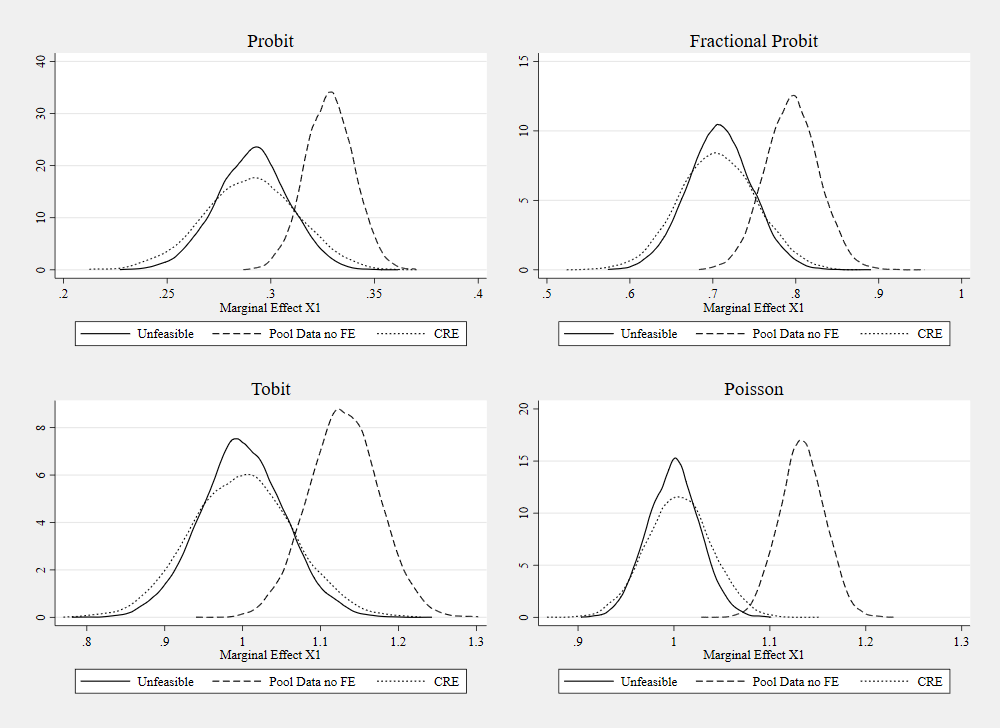
\includegraphics[keepaspectratio]{simulation/fig1.png}}

}

\caption{\label{fig-cre}\emph{Estimated marginal effects/Coefficient
densities for non-linear models}}

\end{figure}%

As expected, the unfeasible estimator, controlling directly for the
unobserved effect \texttt{c1}, provides the benchmark estimates. Since
the unobserved effect \texttt{c1} is correlated with \texttt{x1} and
\texttt{x2} by construction, the pooled estimators (which ignore
\texttt{c1}) exhibit significant bias, as seen in both the density plots
and the summary table.

In contrast, the CRE approach, implemented using the \texttt{cre}
prefix, yields estimates whose distributions are centered close to the
benchmark estimates, indicating negligible bias. While the CRE estimates
show slightly higher variance compared to the unfeasible benchmark (as
reflected in slightly larger MAE in Table~\ref{tbl-cre}), they
effectively mitigate the bias caused by the omitted correlated fixed
effect. This demonstrates the utility of the CRE method for obtaining
consistent estimates in nonlinear panel models where FE is not viable
and RE assumptions are violated.

\begin{table}[H]

\caption{\label{tbl-cre}\emph{Bias and MAE for the estimated marginal
effects/Coefficients for non-linear models}}

\centering{

\{\textless{} include simulation/table1.txt \textgreater\}

}

\end{table}%

\section{Conclusion}\label{sec-6}

This paper introduced \texttt{cre}, a versatile Stata prefix command
designed to simplify the estimation of Correlated Random Effects (CRE)
models based on the Mundlak (1978) specification. The CRE approach
provides a valuable bridge between standard Fixed Effects and Random
Effects models, offering several advantages: it allows for the
estimation of time-invariant variable effects (unlike FE) while
providing consistent estimates for time-varying coefficients even when
the strict RE exogeneity assumption fails (matching FE estimates in
linear models).

The primary contribution of the \texttt{cre} command lies in its
\textbf{flexibility and ease of use}. As a prefix command, it can be
applied to a wide array of Stata's linear and nonlinear estimation
commands, including user-written ones. It automatically handles the
generation of individual means for time-varying covariates, supports
both balanced and unbalanced panels using established methods
\citep{wooldridge2019}, and integrates seamlessly with factor variables
and post-estimation tools like \texttt{margins} for calculating Average
Partial Effects, which is particularly crucial for interpreting
nonlinear models.

We demonstrated through empirical examples that \texttt{cre} replicates
the behavior of specialized commands like \texttt{xtreg,\ cre} in the
linear case while extending functionality to other estimators. For
nonlinear models, we showed how \texttt{cre} provides a practical way to
obtain consistent estimates and APEs, addressing the limitations of FE
and the potentially strong assumptions of RE. Monte Carlo simulations
further confirmed that the CRE approach implemented by \texttt{cre}
effectively reduces bias in nonlinear models with correlated unobserved
effects.

While \texttt{cre} offers a significant simplification for estimating
static CRE models, it currently \textbf{does not address dynamic panel
models}. The inclusion of lagged dependent variables introduces further
econometric challenges (e.g., the initial conditions problem) that
require specialized estimators beyond the scope of this command.

In summary, the \texttt{cre} command provides applied researchers with a
user-friendly and powerful tool for leveraging the benefits of the
Correlated Random Effects approach in Stata, making it easier to
estimate models that account for unobserved heterogeneity while
retaining the ability to analyze the effects of time-invariant
characteristics, especially in nonlinear settings.

\section{Acknowledgments}\label{acknowledgments}

Thanks to Aashima Sinha for her help in the preparation and providing
feedback for this paper, and Enrique Pinzon for his encouragement on
pushing this project forward. I am also grateful to the Editor and an
anonymous referee for their constructive comments on a previous version,
which significantly improved the focus and clarity of this paper.

\clearpage

\bibliographystyle{sj}
\bibliography{references.bib}


\begin{aboutauthors}

Fernando Rios-Avila is an applied econometrician with passion for
econometrics and programming. His research interests include applied
econometrics, labor economics, and poverty and inequality. He has
contributed many commands to Statistical Software Components and written
articles for the Stata Journal.

\end{aboutauthors}

\end{document}
